\chapter{Advanced Driver Assistance Systems}
\label{sec:adas}

This chapter explores and compares several ideas for assistance systems which can be implemented on top of the human driver model generated in the previous one. It starts by tackling the design of the system in terms of the placement in the existing module based model and the capabilities within it, following an incremental approach (considering the limitations of the vehicle and drivers). It then performs a comparison of the different approaches using two distinct test cases and it concludes which ADAS performs the best (within reasonable assumptions). This solution is then evaluated and compared to the human driver in Chapter~\ref{sec:results}.

\section{Driver Assistance System Design}

One of the aims of this dissertation is to obtain correct-by-construction driver assistance systems. As such, the design of the assistance system in this context corresponds mostly to determining which actions are available to the system at each state (the model becomes an MDP), and then performing synthesis using adequate properties. It should be noted that these actions must be realistic in nature, otherwise the obtained assistance system would prove to be useless in a real-world scenario - and usefulness is the end goal in terms of deployment. Figure~\ref{fig:adas_possibilities} presents the underlying assumptions of where the system would lie in the environment, which influences the possibilities in terms of the design.

\vspace{1em}
\begin{figure}[h]
    \centering
    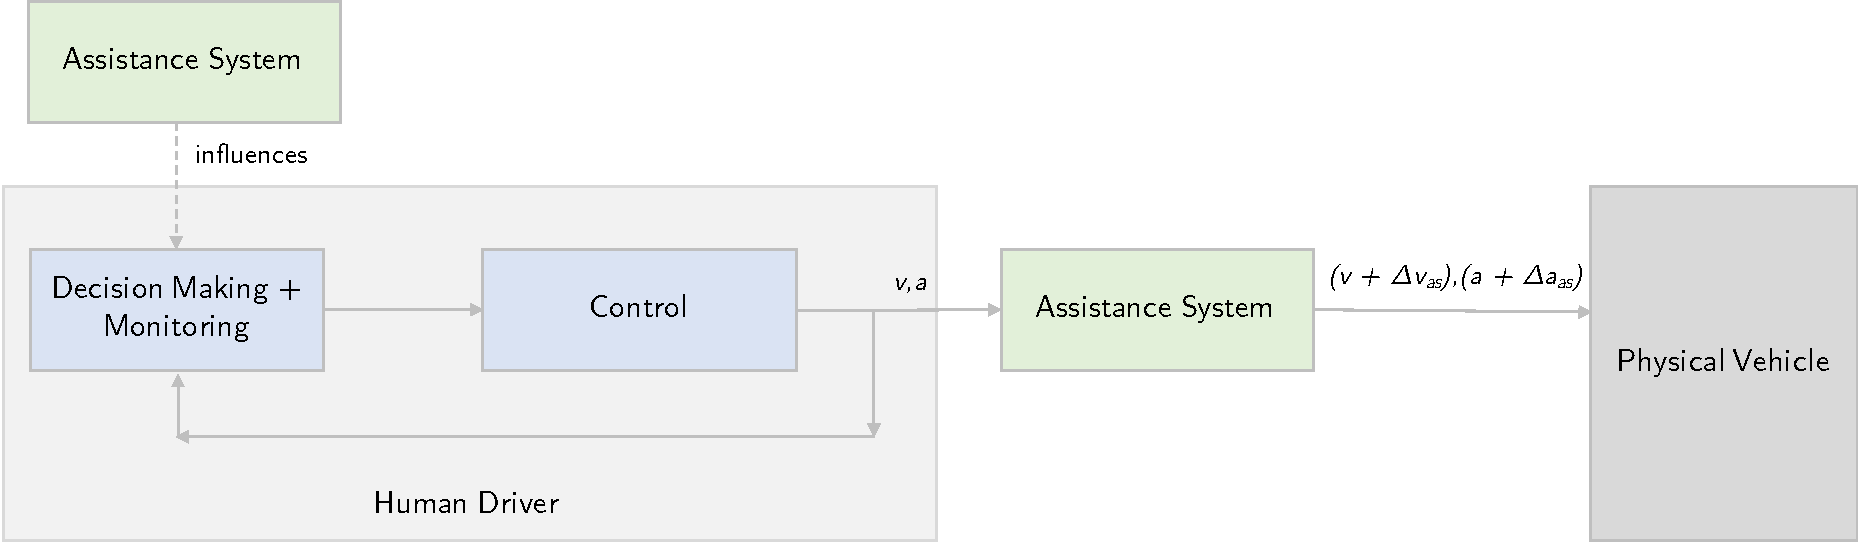
\includegraphics[width=1\textwidth]{adas_possibilities.pdf}
    \caption{Overview of the system with the possibilities of the ADAS intervention.}
    \label{fig:adas_possibilities}
\end{figure}

It is assumed that the assistance system can not change the decision making (as it is a human cognitive process), but it can influence it to a certain degree through suggestion. This would be the ideal way of implementing the ADAS, as it would not require any intervention in the physical systems of the vehicle. Therefore, the first possibilities explored are based on this option. However, in the interest of safety and efficiency, incremental control based options are also developed, both at the level of linear acceleration (influencing $a$ through $\Delta a_{as}$), as well as at the level of steering control (by influencing $v$ and $a$ through $\Delta v_{as}$ and $\Delta a_{as}$, respectively). 

\subsection{Decision Making-based ADAS}

\subsubsection{Decision Making with Fully Compliant Drivers}

At the decision making level, the human driver model considered has two options: it either changes lanes, or it does not. These options can be influenced using suggestions (e.g. through visual or auditive cues) which can lead to either one or the other being taken. Salvucci in \cite{salvucci_1} does not consider accelerating and decelerating as part of the decision making because he argues they happen instinctively and therefore they should be exclusively part of the control. However, if a driver can be influenced to make a conscious decision to decelerate, for example, through the driver assistance system, then there is an argument for including this action in the decision making. Thus, a 3-option ADAS was designed, where an action $\alpha$ is defined as:

\begin{equation}
	\alpha \in A := \{(lc) \vee (\neg lc \wedge a = a_p) \vee (\neg lc \wedge a = a_d)\}
\end{equation}

where $lc$ corresponds to the decision to perform a lane change, $a$ is the acceleration in the next state, $a_p$ is the acceleration the vehicle is currently holding and $a_d$ is a constant value for deceleration that a driver applies when suggested to decelerate. In this dissertation, it was assumed that $a_d = -1$ (minimum decelerating value).

Considering that the drivers are fully compliant with the suggestions given by the system, the decision making at each step can be replaced by the all the possible actions, obtaining an MDP with three choices at this level. The code presented in Appendix~\ref{sec:adas_pdm} corresponds to the implementation of a generator for this ADAS.

\subsubsection{Decision Making with Partially Compliant Drivers}

In the case of the ADAS previously designed, it is assumed that humans will not only follow all the suggestions, but they will comply with them fully and immediately after they are received (within the same ACT-R cycle in the decision making). However, this is not a realistic assumption by any means. In fact, people are more prone to following suggestions when these align with their original intent, than otherwise. With this in mind, a new solution is presented which more accurately represents the suggestive decision making considered in this section.

In the human driver model, a single action was available for a set of conditions, such that at any decision making state ($actr\_state = 2$) $s$ there would be a value $p$ such that the next state $s'$ could be written as:

\begin{equation}
s' = p: (lC) + (1 - p): (\neg lC \:\&\: a = a_p)
\end{equation}

Consider a factor $\gamma \in [0,1]$ which corresponds to how responsive a driver is to the suggestions given. The following rule can be written for each of the actions $\alpha_i \in A$ of the MDP according to the states $s'_i$ which they lead to:

\begin{equation}
s'_i = \gamma: \alpha_i + (1-\gamma)\cdot p:(lC) + (1-\gamma)\cdot (1-p):(\neg lC \:\&\: a = a_p)
\end{equation}

Given that $\gamma, p \in [0,1]$, the transitions are guaranteed to sum up to one for every case. The decision making with fully compliant drivers corresponds to the case where $\gamma = 1$. The code presented in Appendix~\ref{sec:adas_idm} corresponds to the implementation of a generator for this particular ADAS.

\subsection{Control-based ADAS}

While the decision making under the assumption of fully compliant drivers appears to be a powerful option in terms of safety and liveness, the weakening of the assumption to partially compliant drivers is expected to reduce performance substantially, particularly for lower values of $\gamma$. As such, control based assistance is added on top of the decision making assistance considered for partially compliant drivers, so as to improve performance. It should be noted that this type of assistance does not require human intervention, as per the assumptions noted in Figure~\ref{fig:adas_possibilities}.

\subsubsection{Active Linear Acceleration Control}

Considering the assumptions previously described, active linear acceleration control consists in an incremental addition to the acceleration value proposed by the human in the control module. Assume the acceleration of the vehicle imposed by the human is given in the model by $a \in \{a^{\min},...,a^{\max}\}$. In this module, a value $\Delta a_{as}$ is considered such that:

\begin{equation}
\label{eq:delta_as_rest}
	\Delta a_{as} \in \{\Delta a_{as}^{\min},...,\Delta a_{as}^{\min}\}: \Delta a_{as}^{\min} > a^{\min} \wedge \Delta a_{as}^{\max} < a^{\max}
\end{equation}

and the final acceleration applied to the vehicle becomes (considering as well that $a' \in \{a^{\min},...,a^{\max}\}$):

\begin{equation}
	a'(t) = \max (\min (a(t) + \Delta a_{as}, a^{\max}), a^{\min})
\end{equation}

The restriction to the values of $\Delta a_{as}$ presented in Equation~\ref{eq:delta_as_rest} allows the system to be incremental (i.e. corrective) instead of enforcing the specific values chosen by the control assistance system. This is important to avoid strategies for the control assistance system which sharply contrast in terms of the values chosen, e.g. a strategy which at a certain time chooses an acceleration of $3$ and in the next time step chooses one of $-2$ (not allowed for a small enough range of $\Delta a_{as}$ and according to the linear control abstraction obtained in Chapter~\ref{sec:human_driver}). In this dissertation, it is assumed that $\Delta a_{as} \in \{-1,0,1\}$.

The implementation of such system consists in replacing the existing linear control at each step of the control module by the resulting accelerations of applying all the possible values of $\Delta a_{as}$ to the acceleration decided by the human control module, obtaining an MDP with at most three actions at the linear acceleration control level (and at least two). The code presented in Appendix~\ref{sec:adas_lc} corresponds to the implementation of a generator for this ADAS (with the decision making assistance for partially compliant drivers).

\subsubsection{Active Steering Control}

While linear acceleration control assistance improves safety and liveness, steering assistance can also be improved using incremental velocity and acceleration. 

In \cite{salvucci_1}, Salvucci introduces a control law for the steering angle $\varphi$, as presented in Section~\ref{sec:salvucci}, for a given $k_{far}, k_{near}$ and $k_I$. By changing the values of these constants, different control laws are obtained, which introduce different accelerations and velocities at each time step, mimicking the behaviour of the incremental control previously assumed (i.e. within such a strategy, the difference in acceleration and velocity introduced is the difference between these values for the two control laws at each time step). The value of $\theta_{\max}$ (as defined in Section~\ref{sec:salvucci}), guarantees the feasibility of the movement in terms of the acceleration induced. Thus, actions in this assistance system at the model level correspond to different sets of $(k_{far}, k_{near},k_I)$ available to the ADAS.

In this dissertation, three distinct sets of parameters were considered as possible actions, $(k_{far}, k_{near},k_I) \in \{(15,3,5), (17,3,6), (14.5,3,7)\}$. An example of the simulation for the situation where $o_{lane} = 1$, $d = 20m$, $v = 15m/s$ and $v_1 = 15m/s$ (with the non-probabilistic control) is presented in Figure~\ref{fig:steering_control_ex}.

\begin{figure}[h]
    \centering
    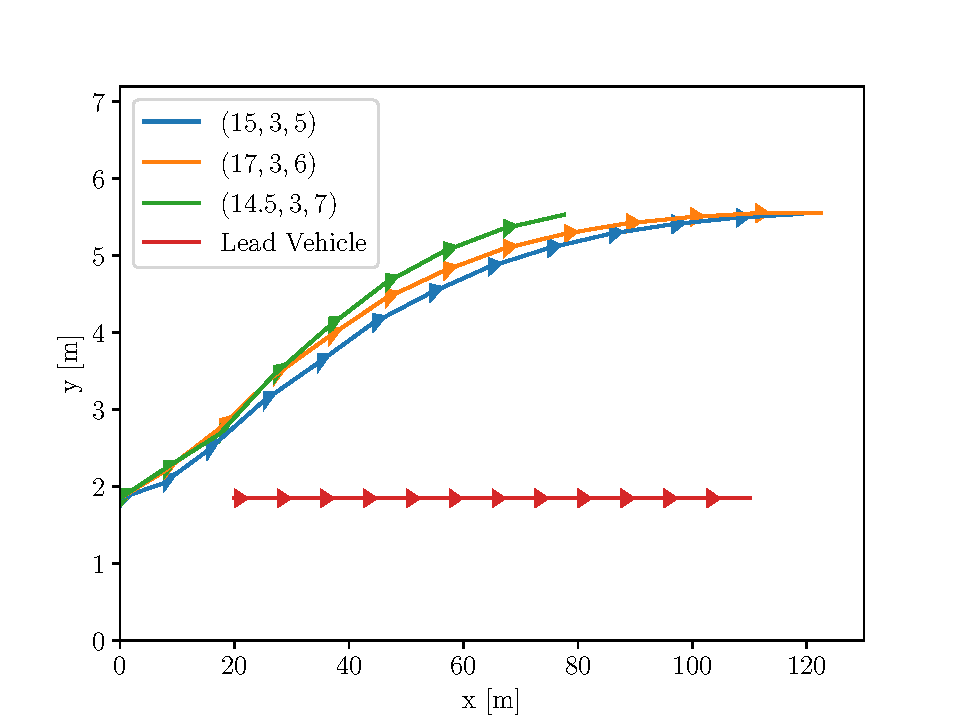
\includegraphics[width=0.9\textwidth]{steering_control_ex.pdf}
    \caption{Example of the simulation of the lane change for $o_{lane} = 1$ (right lane), $d = 20m$, $v = 15m/s$ and $v_1 = 15m/s$ (the legend of each path corresponds to the situation with parameters $k_{far}, k_{near},k_I$, respectively).}
    \label{fig:steering_control_ex}
\end{figure}

Using these values, new look-up tables were obtained with the probability of crashing, the $\Delta x$ and $\Delta T$ incurred and the final velocity of the vehicle in question (following the probabilistic control module presented in Section~\ref{sec:prob_control}) for each origin lane, distance to the other vehicle, velocities of both the vehicle in question and the other vehicle and the parameters of the control law (out of the three possibilities presented). Following the same calculations as shown in Section~\ref{sec:non_prob_control}, the obtained look-up table contains $103,200$ rows.

In terms of implementation, the MDP is obtained through simply reading the three possible actions for lane changing directly from the look-up table, similarly to the human driver model (the difference being the latter only has one option). The code presented in Appendix~\ref{sec:adas_sc} corresponds to the implementation of a generator for this ADAS (with the decision making assistance for partially compliant drivers and active linear acceleration control).

\section{Design Evaluation}

While it would appear to be the case that an ADAS with both decision making and control assistance at the linear acceleration and steering level would be the optimal choice for the driver assistance system, there are no guarantees that this is true. As such, an evaluation and comparison of all the possible designs must be performed in order to determine the best option which can then be compared to the human driver model in Chapter~\ref{sec:results}. To do so, it is necessary to establish multi-objective metrics and some meaningful test cases (as testing all the options would be infeasible).

\subsection{Multi-Objective Metrics}
\label{sec:multi_obj_metrics}

As established in Section~\ref{sec:model_metrics}, safety and liveness are two important metrics which will be used in Chapter~\ref{sec:results} to evaluate the human driver model. Therefore, it makes sense that such properties should be the focus of the synthesis for the driver assistance system. The goal is to minimise the probability of crashing and to maximise the liveness property. This can be obtained using a multi-objective query such as the one below:

\begin{minipage}{\linewidth}
{\vspace{1em}
\begin{lstlisting}
multi(Pmin=? [F crashed], Pmax=? [F (x=length) & (t<T)])
\end{lstlisting}
}
\end{minipage}

for a given constant $T$. Due to the trade-offs between both properties, the model checking of the multi-objective property of the format of the above generates a Pareto curve, where each point on the curve corresponds to optimal achievable values in terms of \texttt{P=? [F crashed]} and \texttt{P=? [F (x=500) \& (t<T)]} under a given strategy. As such, it is possible to compare strategies through the comparison of the Pareto curves obtained for the different ADAS for some test cases.

However, the problem of the safety bias discussed in Section~\ref{sec:live_props} persists through this comparison, and the ideal metric would take into account the conditional probability instead of the unconditional one. Since PRISM does not allow for the model checking of conditional properties, the Pareto curve using the conditional properties needs to be obtained in a different way. At this point, it is important to notice the following equality for a given strategy $\sigma$ in the MDP:

\begin{equation}
	P^{\sigma}_s (\text{\texttt{F crashed}}) = 1 - P^{\sigma}_s (\text{\texttt{F x=length}})
\end{equation}

as long as $p_{\max, s} (\text{\texttt{F (crashed | x = length)}}) = p_{\min, s} (\text{\texttt{F (crashed | x = length)}}) = 1$ (completeness property for the MDP). This is true from the fact that the events crashing and reaching the end are mutually exclusive. Thus, it is possible to write:

\begin{equation}
\label{eq:bayes}
\begin{aligned}
	P^{\sigma}_s (\text{\texttt{F (x=length) \& (t<T)}} \bigmid \text{\texttt{F x=length}}) & = \frac{P^{\sigma}_s (\text{\texttt{F (x=length) \& (t<T)}})}{P^{\sigma}_s (\text{\texttt{F x=length}})} \\
	&  = \frac{P^{\sigma}_s (\text{\texttt{F (x=length) \& (t<T)}})}{1 - P^{\sigma}_s (\text{\texttt{F crashed}})}
\end{aligned}
\end{equation}

It is therefore possible to obtain the Pareto curve with the conditional properties by using Equation~\ref{eq:bayes} on each of the points in the unconditional curve (generating the achievable set through this).

\subsection{Test Cases}

Due to the infeasibility of generating all the possible combinations of test cases, two test cases were considered when comparing the four different ADAS designed in the previous section: the first test case in the scenario $(v, v_1, x_{1,0}) = (21, 19, 70)$ and the second in the scenario $(v, v_1, x_{1,0}) = (30, 22, 50)$. For each of these test cases, the unconditional and conditional Pareto curves for each driver type are presented for a $T$ representative of the scenario and which allows for comparison between the ADAS considered, with Figures~\ref{fig:test_case_1_uncond} and \ref{fig:test_case_1_cond} referring to the first test case, and Figures~\ref{fig:test_case_2_uncond} and \ref{fig:test_case_2_cond} referring to the second test case. In terms of parameters of the model, the same values were used as in the human driver model part of the implementation, and $\gamma$ was set to 0.1.

%For the sake of brevity, the following numbering will be assumed in the captions and discussion of the Pareto curves presented in the test cases:
%
%\begin{enumerate}
%	\item Decision making based ADAS with fully compliant drivers
%	\item Decision making based ADAS with partially compliant drivers (varies with classes of drivers)
%	\item Decision making with partially compliant drivers + linear acceleration control ADAS (varies with classes of drivers)
%	\item Decision making with partially compliant drivers + linear acceleration control + steering control ADAS (varies with classes of drivers)
%\end{enumerate}

%\subsubsection{$v = 21$ m/s, $v_1 = 19$ m/s, $x_{1,0} = 70$ m ($T=20$)}

\begin{figure}[H]
\centering
\begin{subfigure}{0.32\textwidth}
  \centering
  \includegraphics[width=1\textwidth]{test_cases/21_19_70/uncond/1.pdf}
  \subcaption{(1)}
\end{subfigure}\\
\begin{subfigure}{0.32\textwidth}
  \centering
  \includegraphics[width=1\textwidth]{test_cases/21_19_70/uncond/2_1.pdf}
  \subcaption{(2) - Aggressive drivers}
\end{subfigure} 
\begin{subfigure}{0.32\textwidth}
  \centering
  \includegraphics[width=1\textwidth]{test_cases/21_19_70/uncond/2_2.pdf}
  \subcaption{(2) - Average drivers}
\end{subfigure}
\begin{subfigure}{0.32\textwidth}
  \centering
  \includegraphics[width=1\textwidth]{test_cases/21_19_70/uncond/2_3.pdf}
  \subcaption{(2) - Cautious drivers}
\end{subfigure}
\begin{subfigure}{0.32\textwidth}
  \centering
  \includegraphics[width=1\textwidth]{test_cases/21_19_70/uncond/3_1.pdf}
  \subcaption{(3) - Aggressive drivers}
\end{subfigure}
\begin{subfigure}{0.32\textwidth}
  \centering
  \includegraphics[width=1\textwidth]{test_cases/21_19_70/uncond/3_2.pdf}
  \subcaption{(3) - Average drivers}
\end{subfigure}
\begin{subfigure}{0.32\textwidth}
  \centering
  \includegraphics[width=1\textwidth]{test_cases/21_19_70/uncond/3_3.pdf}
  \subcaption{(3) - Cautious drivers}
\end{subfigure}
\begin{subfigure}{0.32\textwidth}
  \centering
  \includegraphics[width=1\textwidth]{test_cases/21_19_70/uncond/4_1.pdf}
  \subcaption{(4) - Aggressive drivers}
\end{subfigure} 
\begin{subfigure}{0.32\textwidth}
  \centering
  \includegraphics[width=1\textwidth]{test_cases/21_19_70/uncond/4_2.pdf}
  \subcaption{(4) - Average drivers}
\end{subfigure}
\begin{subfigure}{0.32\textwidth}
  \centering
  \includegraphics[width=1\textwidth]{test_cases/21_19_70/uncond/4_3.pdf}
  \subcaption{(4) - Cautious drivers}
\end{subfigure}
\caption{Pareto curves of the unconditional properties for the scenario $v = 21m/s$, $v_1 = 19m/s$, $x_{1,0} = 70m$ and for $T = 20$. The ADAS are represented using the following numbering: (1) decision making-based with fully compliant drivers, (2) decision making-based with partially compliant drivers, (3) decision making with partially compliant drivers + linear acceleration control, and (4) decision making with partially compliant drivers + linear acceleration control + steering control.}
\label{fig:test_case_1_uncond}
\end{figure}

%\begin{figure}[H] \ContinuedFloat
%\centering
%\begin{subfigure}{0.49\textwidth}
%  \centering
%  \includegraphics[width=1\textwidth]{test_cases/21_19_70/uncond/3_3.pdf}
%  \subcaption{3 (Cautious drivers)}
%\end{subfigure}
%\begin{subfigure}{0.49\textwidth}
%  \centering
%  \includegraphics[width=1\textwidth]{test_cases/21_19_70/uncond/4_1.pdf}
%  \subcaption{4 (Aggressive drivers)}
%\end{subfigure} 
%\begin{subfigure}{0.49\textwidth}
%  \centering
%  \includegraphics[width=1\textwidth]{test_cases/21_19_70/uncond/4_2.pdf}
%  \subcaption{4 (Average drivers)}
%\end{subfigure}
%\begin{subfigure}{0.49\textwidth}
%  \centering
%  \includegraphics[width=1\textwidth]{test_cases/21_19_70/uncond/4_3.pdf}
%  \subcaption{4 (Cautious drivers)}
%\end{subfigure}
%\caption{Pareto curves for the unconditional properties, for $T = 20$ (cont.).}
%\end{figure}

\begin{figure}[H]
%\vspace{3em}
\centering
\begin{subfigure}{0.32\textwidth}
  \centering
  \includegraphics[width=1\textwidth]{test_cases/21_19_70/cond/1.pdf}
  \subcaption{(1)}
\end{subfigure}\\
\begin{subfigure}{0.32\textwidth}
  \centering
  \includegraphics[width=1\textwidth]{test_cases/21_19_70/cond/2_1.pdf}
  \subcaption{(2) - Aggressive drivers}
\end{subfigure} 
\begin{subfigure}{0.32\textwidth}
  \centering
  \includegraphics[width=1\textwidth]{test_cases/21_19_70/cond/2_2.pdf}
  \subcaption{(2) - Average drivers}
\end{subfigure}
\begin{subfigure}{0.32\textwidth}
  \centering
  \includegraphics[width=1\textwidth]{test_cases/21_19_70/cond/2_3.pdf}
  \subcaption{(2) - Cautious drivers}
\end{subfigure}
\begin{subfigure}{0.32\textwidth}
  \centering
  \includegraphics[width=1\textwidth]{test_cases/21_19_70/cond/3_1.pdf}
  \subcaption{(3) - Aggressive drivers}
\end{subfigure}
\begin{subfigure}{0.32\textwidth}
  \centering
  \includegraphics[width=1\textwidth]{test_cases/21_19_70/cond/3_2.pdf}
  \subcaption{(3) - Average drivers}
\end{subfigure}
\begin{subfigure}{0.32\textwidth}
  \centering
  \includegraphics[width=1\textwidth]{test_cases/21_19_70/cond/3_3.pdf}
  \subcaption{(3) - Cautious drivers}
\end{subfigure}
\begin{subfigure}{0.32\textwidth}
  \centering
  \includegraphics[width=1\textwidth]{test_cases/21_19_70/cond/4_1.pdf}
  \subcaption{(4) - Aggressive drivers}
\end{subfigure} 
\begin{subfigure}{0.32\textwidth}
  \centering
  \includegraphics[width=1\textwidth]{test_cases/21_19_70/cond/4_2.pdf}
  \subcaption{(4) - Average drivers}
\end{subfigure}
\begin{subfigure}{0.32\textwidth}
  \centering
  \includegraphics[width=1\textwidth]{test_cases/21_19_70/cond/4_3.pdf}
  \subcaption{(4) - Cautious drivers}
\end{subfigure}
\caption{Pareto curves of the conditional properties for the scenario $v = 21m/s$, $v_1 = 19m/s$, $x_{1,0} = 70m$ and for $T = 20$. The ADAS are represented using the following numbering: (1) decision making-based with fully compliant drivers, (2) decision making-based with partially compliant drivers, (3) decision making with partially compliant drivers + linear acceleration control, and (4) decision making with partially compliant drivers + linear acceleration control + steering control.}
\label{fig:test_case_1_cond}
\end{figure}

%\begin{figure}[H] \ContinuedFloat
%\centering
%\begin{subfigure}{0.49\textwidth}
%  \centering
%  \includegraphics[width=1\textwidth]{test_cases/21_19_70/cond/3_3.pdf}
%  \subcaption{3 (Cautious drivers)}
%\end{subfigure}
%\begin{subfigure}{0.49\textwidth}
%  \centering
%  \includegraphics[width=1\textwidth]{test_cases/21_19_70/cond/4_1.pdf}
%  \subcaption{4 (Aggressive drivers)}
%\end{subfigure} 
%\begin{subfigure}{0.49\textwidth}
%  \centering
%  \includegraphics[width=1\textwidth]{test_cases/21_19_70/cond/4_2.pdf}
%  \subcaption{4 (Average drivers)}
%\end{subfigure}
%\begin{subfigure}{0.49\textwidth}
%  \centering
%  \includegraphics[width=1\textwidth]{test_cases/21_19_70/cond/4_3.pdf}
%  \subcaption{4 (Cautious drivers)}
%\end{subfigure}
%\caption{Pareto curves for the conditional properties, for $T = 20$ (cont.).}
%\end{figure}

%\subsubsection{$v = 30$ m/s, $v_1 = 22$ m/s, $x_{1,0} = 50$ m ($T=19$)}

\begin{figure}[H]
%\vspace{3em}
\centering
\begin{subfigure}{0.32\textwidth}
  \centering
  \includegraphics[width=1\textwidth]{test_cases/30_22_50/uncond/1.pdf}
  \subcaption{(1)}
\end{subfigure}\\
\begin{subfigure}{0.32\textwidth}
  \centering
  \includegraphics[width=1\textwidth]{test_cases/30_22_50/uncond/2_1.pdf}
  \subcaption{(2) - Aggressive drivers}
\end{subfigure} 
\begin{subfigure}{0.32\textwidth}
  \centering
  \includegraphics[width=1\textwidth]{test_cases/30_22_50/uncond/2_2.pdf}
  \subcaption{(2) - Average drivers}
\end{subfigure}
\begin{subfigure}{0.32\textwidth}
  \centering
  \includegraphics[width=1\textwidth]{test_cases/30_22_50/uncond/2_3.pdf}
  \subcaption{(2) - Cautious drivers}
\end{subfigure}
\begin{subfigure}{0.32\textwidth}
  \centering
  \includegraphics[width=1\textwidth]{test_cases/30_22_50/uncond/3_1.pdf}
  \subcaption{(3) - Aggressive drivers}
\end{subfigure}
\begin{subfigure}{0.32\textwidth}
  \centering
  \includegraphics[width=1\textwidth]{test_cases/30_22_50/uncond/3_2.pdf}
  \subcaption{(3) - Average drivers}
\end{subfigure}
\begin{subfigure}{0.32\textwidth}
  \centering
  \includegraphics[width=1\textwidth]{test_cases/30_22_50/uncond/3_3.pdf}
  \subcaption{(3) - Cautious drivers}
\end{subfigure}
\begin{subfigure}{0.32\textwidth}
  \centering
  \includegraphics[width=1\textwidth]{test_cases/30_22_50/uncond/4_1.pdf}
  \subcaption{(4) - Aggressive drivers}
\end{subfigure} 
\begin{subfigure}{0.32\textwidth}
  \centering
  \includegraphics[width=1\textwidth]{test_cases/30_22_50/uncond/4_2.pdf}
  \subcaption{(4) - Average drivers}
\end{subfigure}
\begin{subfigure}{0.32\textwidth}
  \centering
  \includegraphics[width=1\textwidth]{test_cases/30_22_50/uncond/4_3.pdf}
  \subcaption{(4) - Cautious drivers}
\end{subfigure}
\caption{Pareto curves of the unconditional properties for the scenario $v = 30m/s$, $v_1 = 22m/s$, $x_{1,0} = 50m$ and for $T = 19$. The ADAS are represented using the following numbering: (1) decision making-based with fully compliant drivers, (2) decision making-based with partially compliant drivers, (3) decision making with partially compliant drivers + linear acceleration control, and (4) decision making with partially compliant drivers + linear acceleration control + steering control.}
\label{fig:test_case_2_uncond}
\end{figure}

%\begin{figure}[H] \ContinuedFloat
%\centering
%\begin{subfigure}{0.49\textwidth}
%  \centering
%  \includegraphics[width=1\textwidth]{test_cases/30_22_50/uncond/3_3.pdf}
%  \subcaption{3 (Cautious drivers)}
%\end{subfigure}
%\begin{subfigure}{0.49\textwidth}
%  \centering
%  \includegraphics[width=1\textwidth]{test_cases/30_22_50/uncond/4_1.pdf}
%  \subcaption{4 (Aggressive drivers)}
%\end{subfigure} 
%\begin{subfigure}{0.49\textwidth}
%  \centering
%  \includegraphics[width=1\textwidth]{test_cases/30_22_50/uncond/4_2.pdf}
%  \subcaption{4 (Average drivers)}
%\end{subfigure}
%\begin{subfigure}{0.49\textwidth}
%  \centering
%  \includegraphics[width=1\textwidth]{test_cases/30_22_50/uncond/4_3.pdf}
%  \subcaption{4 (Cautious drivers)}
%\end{subfigure}
%\caption{Pareto curves for the unconditional properties, for $T = 19$ (cont.).}
%\label{fig:test_case_2_uncond}
%\end{figure}

\begin{figure}[H]
\vspace{3em}
\centering
\begin{subfigure}{0.32\textwidth}
  \centering
  \includegraphics[width=1\textwidth]{test_cases/30_22_50/cond/1.pdf}
  \subcaption{(1)}
\end{subfigure}\\
\begin{subfigure}{0.32\textwidth}
  \centering
  \includegraphics[width=1\textwidth]{test_cases/30_22_50/cond/2_1.pdf}
  \subcaption{(2) - Aggressive drivers}
\end{subfigure} 
\begin{subfigure}{0.32\textwidth}
  \centering
  \includegraphics[width=1\textwidth]{test_cases/30_22_50/cond/2_2.pdf}
  \subcaption{(2) - Average drivers}
\end{subfigure}
\begin{subfigure}{0.32\textwidth}
  \centering
  \includegraphics[width=1\textwidth]{test_cases/30_22_50/cond/2_3.pdf}
  \subcaption{(2) - Cautious drivers}
\end{subfigure}
\begin{subfigure}{0.32\textwidth}
  \centering
  \includegraphics[width=1\textwidth]{test_cases/30_22_50/cond/3_1.pdf}
  \subcaption{(3) - Aggressive drivers}
\end{subfigure}
\begin{subfigure}{0.32\textwidth}
  \centering
  \includegraphics[width=1\textwidth]{test_cases/30_22_50/cond/3_2.pdf}
  \subcaption{(3) - Average drivers}
\end{subfigure}
\begin{subfigure}{0.32\textwidth}
  \centering
  \includegraphics[width=1\textwidth]{test_cases/30_22_50/cond/3_3.pdf}
  \subcaption{(3) - Cautious drivers}
\end{subfigure}
\begin{subfigure}{0.32\textwidth}
  \centering
  \includegraphics[width=1\textwidth]{test_cases/30_22_50/cond/4_1.pdf}
  \subcaption{(4) - Aggressive drivers}
\end{subfigure} 
\begin{subfigure}{0.32\textwidth}
  \centering
  \includegraphics[width=1\textwidth]{test_cases/30_22_50/cond/4_2.pdf}
  \subcaption{(4) - Average drivers}
\end{subfigure}
\begin{subfigure}{0.32\textwidth}
  \centering
  \includegraphics[width=1\textwidth]{test_cases/30_22_50/cond/4_3.pdf}
  \subcaption{(4) - Cautious drivers}
\end{subfigure}
\caption{Pareto curves of the conditional properties for the scenario $v = 30m/s$, $v_1 = 22m/s$, $x_{1,0} = 50m$ and for $T = 19$. The ADAS are represented using the following numbering: (1) decision making-based with fully compliant drivers, (2) decision making-based with partially compliant drivers, (3) decision making with partially compliant drivers + linear acceleration control, and (4) decision making with partially compliant drivers + linear acceleration control + steering control.}
\label{fig:test_case_2_cond}
\end{figure}

%\begin{figure}[H] \ContinuedFloat
%\centering
%\begin{subfigure}{0.49\textwidth}
%  \centering
%  \includegraphics[width=1\textwidth]{test_cases/30_22_50/cond/3_3.pdf}
%  \subcaption{3 (Cautious drivers)}
%\end{subfigure}
%\begin{subfigure}{0.49\textwidth}
%  \centering
%  \includegraphics[width=1\textwidth]{test_cases/30_22_50/cond/4_1.pdf}
%  \subcaption{4 (Aggressive drivers)}
%\end{subfigure} 
%\begin{subfigure}{0.49\textwidth}
%  \centering
%  \includegraphics[width=1\textwidth]{test_cases/30_22_50/cond/4_2.pdf}
%  \subcaption{4 (Average drivers)}
%\end{subfigure}
%\begin{subfigure}{0.49\textwidth}
%  \centering
%  \includegraphics[width=1\textwidth]{test_cases/30_22_50/cond/4_3.pdf}
%  \subcaption{4 (Cautious drivers)}
%\end{subfigure}
%\caption{Pareto curves for the conditional properties, for $T = 19$ (cont.).}
%\label{fig:test_case_2_cond}
%\end{figure}

\subsection{Overall Comparison}

From the Pareto curves presented, it is noticeable that the best performing ADAS is the first presented, that is, a decision making assistance system with the assumption of fully compliant drivers. This assistance system allows maximum safety (\texttt{P=? [F crashed]} = 0) and efficiency (\texttt{P=? [F (x=500) \& (t<T)]} = 1) for both test cases and respective values of $T$ considered. However, as discussed before, this situation is unrealistic in nature. By adding the partial compliance assumption, the performance drops drastically, leading to fairly high probabilities of crashing in aggressive drivers (minimum of 0.285 for the first test case and 0.294 for the second one) and lower liveness performance as well. By introducing linear acceleration control, safety increases significantly (the probability of crashing is lowered), but the increase of the probability of the liveness property being satisfied is almost negligible in some situations (and it decreases in some cases; e.g. the aggressive drivers in the first test case). In all the cases tested, the introduction of steering control improves, in both cases and for all driver classes, both safety and liveness. Therefore, the assistance system number 4, that is, decision making with partially compliant drivers, active linear acceleration control and active steering control is the best performing system in the two test cases presented (other than number 1, which is based on unrealistic assumptions).

This analysis does not provide a statistical guarantee that this is the best performing ADAS out of the ones tested in the majority of the situations (as this would be too time consuming for the time frame of this dissertation). However, the systems considered are incremental in nature, in the sense that they were built through iteration and by adding more actions to the one immediately before. As such, number 4 was expected for perform better than numbers 2 and 3, simply due to the fact that there were more choices available to it. The two test cases presented corroborate this idea. Therefore, it can be concluded that the assistance system number 4 would be the most complete and better candidate for deployment, and, as such, the in-depth experimental results and discussion presented in Chapter~\ref{sec:results} use this ADAS.
